% Main file for the VolTilt paper (Springer LNCS format, as in DASFAA_2027/samplepaper.tex).
% Build:  latexmk -pdf main.tex   (or pdflatex + bibtex + pdflatex x2). Needs llncs.cls and splncs04.bst, copied next to this file.
% Section files: intro, related_work, problem_formulation, method, experiments, conclusion. Bibliography: references.bib.
% Method figures are included from method.tex: voltilt_arch.pdf (built from voltilt_arch.tex + icons_v10/).
\documentclass[runningheads]{llncs}
%
\usepackage[T1]{fontenc}
\usepackage{newtxtext}
\usepackage[varvw]{newtxmath}
\usepackage{graphicx}   % figures and \resizebox in the tables of experiments.tex
\usepackage{xcolor}
\newcommand{\est}[1]{{\color{red}#1}} % PLACEHOLDER estimate, must be verified (see ESTIMATES_TO_VERIFY.md)
\usepackage{booktabs}   % table rules in experiments.tex
\usepackage{amsmath}    % \mathbb, \operatorname, \eqref
\usepackage{url}
\newcommand{\ieq}[1]{\refstepcounter{equation}\label{#1}\,\textup{(\theequation)}} % inline equation number, keeps \eqref and hyperlinks working
\usepackage{placeins} % \FloatBarrier keeps all tables inside the Experiments section
\usepackage[colorlinks=true,linkcolor=blue,citecolor=blue,urlcolor=blue,bookmarksnumbered=true,pdfusetitle=false]{hyperref} % clickable citations, references and links; load last
%
\begin{document}
%
\title{VolTilt: A Risk-Budgeted LLM Allocator that Separates How Much Risk to Hold from Where to Allocate It}
%
\titlerunning{VolTilt}
%
% TODO: fill in authors and affiliations (remove for double-blind review if required).
\author{First Author\inst{1} \and Second Author\inst{1}}
%
\authorrunning{F. Author et al.}
%
\institute{Institution Name, City, Country\\
\email{author@example.org}}
%
\maketitle
%
\begin{abstract}
An improvement in the risk-adjusted performance of a trading agent can come from the information it extracts from news or from the exposure implied by its allocation rule. We propose VolTilt to examine these contributions. A large language model extracts structured events from financial news, and the ranks of smoothed event scores produce a bounded tilt around equal weights. A volatility-targeting rule scales the invested fraction using realised returns on historically tilted portfolios. The rules for ranking and scaling are distinct, although past tilts can affect today's volatility estimate. We evaluate VolTilt on 13 assets across three benchmarks against a fully invested equal-weight reference, rule-based strategies, and reimplementations of published trading agents. News-off, matched-budget, and shifted-score comparisons assess the incremental contribution of the text signal. Volatility scaling accounts for most of the risk-adjusted gain in the volatile stock window and reduces drawdown. We find little statistically detectable gain from the news tilt, including when the invested fraction is matched across portfolios. Event scores are associated with same-day returns, with little detectable association at forward horizons. Performance for several reimplemented agents varies across backbones.
\keywords{Large language models \and Financial trading agents \and Volatility targeting \and Portfolio allocation.}
\end{abstract}
%
\section{Introduction}

When a trading agent that reads financial news improves its Sharpe ratio, the improvement can come from selecting different assets, holding a different fraction of capital in the market, or both. This ambiguity matters when comparing a news-driven agent with a fully invested reference. An explicit volatility rule and a budget-matched comparison let us examine the contribution of relative asset weights under the same invested fraction.

Large language models (LLMs) can reason over financial text, and prior work has studied whether sentiment extracted from news is associated with subsequent returns~\cite{lopezlira2023chatgpt}. FinMem and TradingGPT use memory to organise information for trading decisions~\cite{yu2024finmem,li2023tradinggpt}. FinCon combines multi-agent decision making with verbal reinforcement~\cite{yu2024fincon}, FinAgent augments its policy with tools~\cite{zhang2024finagent}, and TradingAgents assigns specialised roles to agents~\cite{xiao2024tradingagents}. FLAG-Trader fine-tunes an LLM trading policy through reinforcement learning~\cite{wang2025flagtrader}. When text interpretation feeds directly into a trading policy, changes in the model can affect both asset selection and portfolio exposure, making it difficult to attribute performance to information extracted from news. Benchmark studies document sensitivity to model choice and market conditions~\cite{li2024investorbench,li2025finsaber}. With date-only news, an article may describe a price move that has already occurred. A separate concern is look-ahead through information seen during pretraining~\cite{glasserman2023lookahead,lopezlira2025memorization}.

We propose \textbf{VolTilt}, a long-only allocator that assigns portfolio exposure to an explicit volatility rule and uses an LLM to inform relative asset weights (Section~\ref{sec:method}). The LLM extracts event records under a fixed schema. We retain articles that focus on the asset and report specific figures, smooth their impact scores, and use cross-sectional ranks to form a bounded tilt around equal weights. A common volatility budget scales the allocation using recent realised returns on the tilted portfolio~\cite{moreira2017volmanaged,harvey2018impact}. The text signal can therefore affect the volatility estimate through portfolio composition, while the scaling rule is fixed. Disabling the tilt gives a price-only comparison under the same rule. Holding the resulting budget fixed then lets us compare relative weights at the same daily invested fraction. We evaluate the allocator on three stock and cryptocurrency settings from the FINSABER and InvestorBench benchmarks against a fully invested equal-weight reference, rule-based strategies, and reimplementations of published LLM trading agents~\cite{li2025finsaber,li2024investorbench}.

\noindent\textbf{Our contributions are as follows.}
\begin{itemize}
  \item We develop a long-only allocation method that combines portfolio-level volatility scaling with a bounded rank tilt derived from structured financial news. The fixed event schema allows us to substitute LLM backbones while holding the scoring and allocation rules fixed.
  \item We assess the incremental value of the LLM signal using a price-only ablation, matched daily budgets, shifted-score and article-count controls, and tests of forward return associations under alternative news cutoffs (Section~\ref{sec:experiments}).
  \item We find that volatility scaling improves Sharpe and lowers drawdown relative to equal weight in the FINSABER stock window. The matched-budget comparisons across labellers offer limited evidence that the news tilt improves performance in the two stock settings.
\end{itemize}

\section{Related Work}

\paragraph{LLM trading policies.}
A central problem in LLM-based trading is how to translate heterogeneous financial evidence into portfolio decisions. Memory-based approaches organise information across horizons, as in FinMem and TradingGPT, while FinCon and TradingAgents distribute analysis across specialised agents~\cite{yu2024finmem,li2023tradinggpt,yu2024fincon,xiao2024tradingagents}. FinAgent broadens the evidence available to the policy through tools~\cite{zhang2024finagent}. FLAG-Trader adapts the policy itself through reinforcement learning, extending the use of trading rewards to train financial decision policies~\cite{liu2022finrlmeta,wang2025flagtrader}. These approaches address how trading policies gather evidence and use it to select actions. When evidence processing and position selection are evaluated jointly, however, changes in portfolio performance may reflect either the information extracted from text or the exposures induced by the policy. We therefore identify an attribution gap in measuring the value of the text signal under a common exposure rule.

\paragraph{News signals and return predictability.}
Evaluating a news signal requires distinguishing information about future returns from information about price movements that have already occurred. Studies use LLM-derived sentiment scores and text embeddings to construct signals for return prediction and portfolio sorting~\cite{lopezlira2023chatgpt,kirtac2024sentiment,chen2022expected}. Work on look-ahead bias and memorisation examines a separate threat to inference, namely that a model may have encountered information about the evaluation period during pretraining~\cite{glasserman2023lookahead,lopezlira2025memorization,gao2025lookahead}. Even if pretraining overlap can be ruled out, date-only news leaves the ordering of publication and intraday price changes uncertain. For such data, we regard the incremental value of event scores as unresolved unless forward-return tests distinguish the signal from contemporaneous price movements and from proxies for news volume.

\paragraph{Benchmarking and robustness.}
The reliability of LLM trading policies is difficult to assess when results depend on the model backbone, market conditions, or the information supplied to the agent. InvestorBench facilitates comparisons under common tasks across assets and backbones, while FINSABER examines performance over longer horizons and across market conditions~\cite{li2024investorbench,li2025finsaber}. AutoRedTrader tests sensitivity to misleading financial news~\cite{liu2026autoredtrader}, while TradeTrap stress-tests components of the trading pipeline~\cite{tradetrap2025}. These evaluations address different sources of variation, but a change in strategy performance after a backbone substitution may reflect changes in both text interpretation and exposure. The remaining question is how much backbone sensitivity persists when the exposure rule is held fixed.

\paragraph{Volatility-managed portfolios.}
Changes in realised volatility can leave portfolios with substantially different levels of risk over time. Volatility management addresses this problem by reducing exposure when estimated risk rises. Prior work reports improvements in risk-adjusted performance or reductions in downside risk for some portfolios, although gains can weaken under implementable out-of-sample rules~\cite{moreira2017volmanaged,harvey2018impact,cederburg2020volmanaged}. Guidance on backtest design also highlights the risk of attributing gains to a rule selected using the evaluation data~\cite{lopezdeprado2018advances}. For a news-based strategy, we therefore ask whether the signal improves risk-adjusted performance relative to a price-only allocation subject to the same volatility rule.

\section{Problem Formulation}
\label{sec:problem}

An LLM trading policy can change both the assets a portfolio holds and the fraction of capital it invests. A higher Sharpe ratio or a shallower drawdown can therefore reflect better asset ranking, a change in aggregate exposure, or the interaction between the two. We ask whether an LLM-derived news signal adds value once we account for the portfolio's volatility-control rule.

\subsection{Information and Decision Timing}

We consider daily allocation over a universe of $N$ stocks or cryptocurrencies. Let $p_{i,t}$ be the adjusted closing price of asset $i$ on panel date $t$, and let $\mathcal{A}_t$ be the set of assets with a valid close on that date, with $N_t=|\mathcal{A}_t|$. For adjacent closes the return ending at $t+1$ is $r_{i,t+1}=p_{i,t+1}/p_{i,t}-1$. We write $\mathcal{X}_{i,t}$ for the news items associated with asset $i$ and dated $t$. The allocator selects positions at the close using $\mathcal{F}_t=\{p_{i,s},\mathcal{X}_{i,s}:s\leq t\}$, with missing inputs allowed, for the subsequent holding interval.

We use data from FINSABER and InvestorBench~\cite{li2025finsaber,li2024investorbench}. When an item has only a date, we treat it as available at that day’s close. The backtest also uses the final close in the decision, so same-close execution is an alignment assumption for both inputs. In Section~\ref{sec:experiments} we delay news by one observed session and separately test trading one session after forming the entire target portfolio. These timing checks address information availability at execution. Pretraining overlap poses a separate source of look-ahead.

\subsection{Capital Weights and Backtest Accounting}

We write $q_{i,t}$ for the share of invested capital assigned to asset $i$ and $\lambda_t$ for the total invested fraction. The target capital weights, including the uninvested fraction $a_{0,t}$, satisfy
$a_{i,t}=\lambda_t q_{i,t}=w_{i,t}/N_t$, $q_{i,t}\geq 0$, $\sum_{i\in\mathcal{A}_t} q_{i,t}=1$, $0\leq\lambda_t\leq1$, and $a_{0,t}=1-\lambda_t$~\ieq{eq:capital-weights}.
Here $w_{i,t}$ is the exposure multiplier relative to the equal capital share $1/N_t$. Cash earns zero in the backtest.

The main portfolio backtest tracks returns and changes in multipliers by asset. Let $t_i^+$ and $t_i^-$ be the next and preceding observed closes of asset $i$ around $t$, and let $\mathcal{D}_t(\pi)$ be the legs with both a recorded position under policy $\pi$ at $t$ and a subsequent observed close. The net return observation indexed by decision date $t$ is
\begin{equation}
  R^{\mathrm{net}}_t(\pi)
    =\frac{1}{|\mathcal{D}_t(\pi)|}
      \sum_{i\in\mathcal{D}_t(\pi)}\!
        \left[w_{i,t}\left(\frac{p_{i,t_i^+}}{p_{i,t}}-1\right)
            -c\,|w_{i,t}-w_{i,t_i^-}|\right].
  \label{eq:portret}
\end{equation}
We omit dates with no realised legs. The cost proxy uses zero for the initial or missing preceding multiplier. On a complete panel the return term is the usual weighted sum with capital weights $a_{i,t}$. With missing observations, the implementation averages realised legs only. An intervening gap extends the interval to the next observed close, and a leg with no subsequent close contributes no return or separate liquidation adjustment. This ex-post averaging can change the effective denominator relative to the target allocation. The cost term averages absolute changes in target multipliers over those same legs. It omits price drift and turnover due solely to a change in the number of eligible assets. Our fully invested equal-weight reference uses $w_{i,t}=1$ on each eligible asset and thus targets equal shares at each close.

\subsection{Attribution Contrasts}

Let $\boldsymbol{q}^{\mathrm{news}}$ be the sequence of news-derived relative weights and let $\boldsymbol{q}^{\mathrm{eq}}$ assign $q^{\mathrm{eq}}_{i,t}=1/N_t$. Applying the same volatility rule to the history of each allocation gives the budget sequences $\boldsymbol{\lambda}^{\mathrm{news}}$ and $\boldsymbol{\lambda}^{\mathrm{eq}}$. With $\mathrm{SR}(\boldsymbol{\lambda},\boldsymbol{q})$ denoting annualised Sharpe on aligned dates under common cost accounting, we define the incremental policy contrast
\begin{equation}
  \Delta_{\mathrm{policy}}=
    \mathrm{SR}(\boldsymbol{\lambda}^{\mathrm{news}},\boldsymbol{q}^{\mathrm{news}})
    -\mathrm{SR}(\boldsymbol{\lambda}^{\mathrm{eq}},\boldsymbol{q}^{\mathrm{eq}}).
  \label{eq:policy-contrast}
\end{equation}
This contrast allows the budget to respond to historical composition. To measure the change in relative weights at the same daily invested fraction, we also use
\begin{equation}
  \Delta_{\mathrm{comp}}(\boldsymbol{\lambda}^{\mathrm{ref}})=
    \mathrm{SR}(\boldsymbol{\lambda}^{\mathrm{ref}},\boldsymbol{q}^{\mathrm{news}})
    -\mathrm{SR}(\boldsymbol{\lambda}^{\mathrm{ref}},\boldsymbol{q}^{\mathrm{eq}}).
  \label{eq:composition-contrast}
\end{equation}
We take $\boldsymbol{\lambda}^{\mathrm{ref}}=\boldsymbol{\lambda}^{\mathrm{eq}}$, computed from information available at each decision. This retrospective comparison holds the daily invested fraction constant. The compositions can still differ in turnover, realised volatility, and factor exposures, so the contrast measures the net portfolio effect of reallocating capital at the chosen budget.

\subsection{Performance and News Information}

We use annualised net Sharpe as the primary performance measure and report cumulative return, realised volatility, and maximum drawdown alongside it. Section~\ref{sec:experiments} specifies the benchmark windows and inference procedures. We separately test the association between the unsmoothed daily event score $h_{i,t}$ in Eq.~\eqref{eq:vt-score} and subsequent returns. For this diagnostic, $t$ indexes each asset's observed sessions, with $Y^{(0)}_{i,t}=p_{i,t}/p_{i,t-1}-1$ and $Y^{(h)}_{i,t}=p_{i,t+h}/p_{i,t}-1$ for $h\in\{1,5\}$. We rank each variable within each asset over its included sessions, then compute the Pearson correlation over the pooled asset--session pairs:
\begin{equation}
  \mathrm{IC}_h=\operatorname{Corr}_{(i,t)}
     \bigl(\operatorname{PctRank}_i(h_{i,t}),
           \operatorname{PctRank}_i(Y^{(h)}_{i,t})\bigr).
  \label{eq:ic}
\end{equation}
The same-day coefficient measures contemporaneous association. In particular, dated news can describe a price movement that has already occurred by the close. The forward coefficients use cumulative returns from the decision close through the next one or five observed sessions. We also test the signal that drives the traded ranks. For each eligible date in a stock window, we compute Spearman correlation across assets between $s_{i,t}$ and the forward return, then average these daily correlations. Section~\ref{sec:experiments} describes eligibility, ties, and inference.

\section{Method}
\label{sec:method}

VolTilt uses two rules to construct the allocation in Section~\ref{sec:problem}. An LLM reads financial news and produces event records from which we derive the relative shares $q_{i,t}$. A volatility-targeting rule converts historical portfolio returns into the invested fraction $\lambda_t$ (Fig.~\ref{fig:overview}). We express the relative shares using the rank multiplier $\tau_{i,t}$ so that the capital weight is $a_{i,t}=\lambda_t q_{i,t}=\lambda_t\tau_{i,t}/N_t$. The exposure multiplier recorded by the backtest is $w_{i,t}=N_t a_{i,t}$. A backbone can be substituted through the event-record schema while the allocation rules remain fixed. Past news can still influence the invested fraction through the historical tilts used to estimate volatility.

\begin{figure}[tb]
\centering
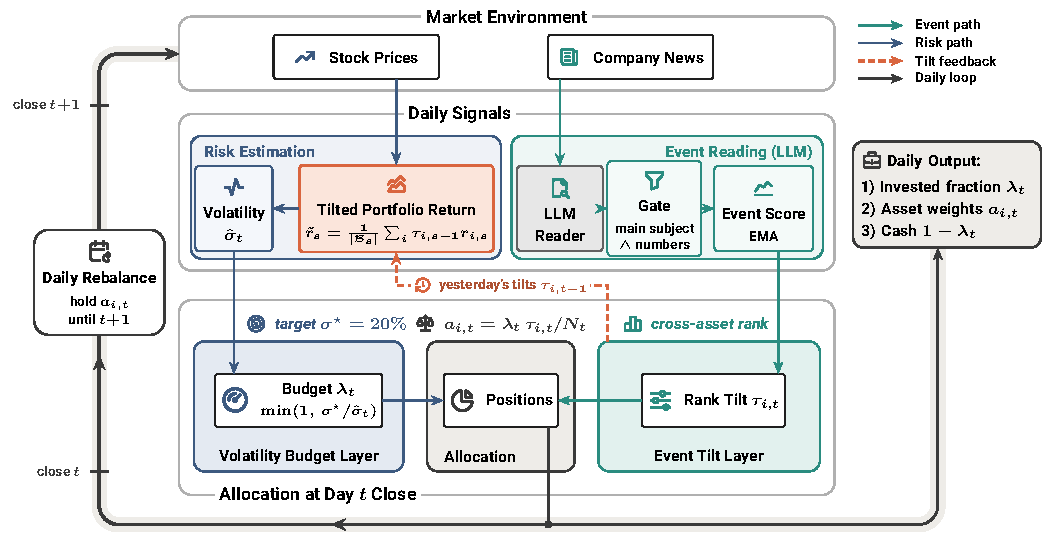
\includegraphics[width=\textwidth]{voltilt_arch.pdf}
\caption{VolTilt allocation at close $t$. The event path ranks smoothed news scores to set relative weights. The risk path scales invested capital using recent volatility. The dashed connection shows how past tilts enter the risk estimate through realised returns. We hold positions until the next rebalance.}
\label{fig:overview}
\end{figure}

\subsection{Structured Event Scoring}

For each asset--article pair, the LLM receives the company name and the first $1{,}500$ characters of the cleaned article. At temperature zero, it produces a record with five fields: \texttt{focus}, \texttt{event\_type}, \texttt{novelty}, \texttt{hard\_numbers}, and \texttt{impact}. The first identifies whether the company is the main subject, is mentioned in passing, or is unrelated. The next two identify one of twelve event categories and distinguish a new fact, follow-up, recap, or opinion. The Boolean \texttt{hard\_numbers} field indicates the presence of company-specific figures. We denote the signed impact by $u_i(x)\in\{-2,-1,0,1,2\}$. The prompt asks for a judgement of the effect of new information over the following week, with zero representing neutral or already-priced information. The prompt instructs the model to use the article alone and judge the impact of new information. The categories cover earnings, guidance, analyst actions, products, legal events, deals, management, supply or demand, aggregate conditions, price recaps, opinions, and other reports. We cache records by the SHA-256 hash of the dataset asset identifier and original article text. Only successfully parsed records enter the score. Articles with missing cache entries contribute nothing.

Let $\mathcal{G}_{i,t}\subseteq\mathcal{X}_{i,t}$ contain the reports that identify the company as the main subject and contain company-specific figures. The gate restricts the signal to company-specific quantitative disclosures. Event type and novelty are retained as metadata. We assess the gate against a main-subject-only control. We sum the impact judgements for the qualifying articles and smooth the daily scores:
$h_{i,t}=\sum_{x\in\mathcal{G}_{i,t}}u_i(x)$ and $s_{i,t}=(1-\alpha)s_{i,t-1}+\alpha h_{i,t}$~\ieq{eq:vt-score}.
We update the EMA once per panel date, including warm-up and dates without qualifying articles, using $s_{i,0}=0$ and $\alpha=2/21$. When $h_{i,t}=0$, the previous score decays. Summation treats increments on the ordinal scale as additive and can give repeated coverage more weight. We compare it with a count-based signal and with averaging the qualifying scores (Section~\ref{sec:experiments}).

\subsection{Bounded Cross-Asset Tilt}

Building on the use of news scores in portfolio weighting~\cite{anic2025systematic}, we use the ordering of the smoothed scores in Eq.~\eqref{eq:vt-score}. The model supplies ordinal impact judgements, and the rank transformation requires no calibration of the scores as expected returns. Let $\rho_{i,t}$ be the ascending rank of $s_{i,t}$ among the $N_t$ assets in $\mathcal{A}_t$, with average ranks for ties. For a universe of at least three assets and at least two eligible assets on day $t$, we set
$\tau_{i,t}=1+k\,\bigl(\rho_{i,t}-(N_t+1)/2\bigr)/\bigl((N_t-1)/2\bigr)$ with $k=0.5$~\ieq{eq:vt-rank}.
We use unit tilts when all scores tie, fewer than two assets are eligible, or the chosen universe contains at most two assets. Ranks discard differences in score magnitude. Small differences can therefore produce different weights, and two distinct scores in a pair would force the full tilt spread. The tilt-off rule for two-asset universes was selected on a design sample. Section~\ref{sec:experiments} describes that selection and tests sensitivity to the fixed tilt strength $k$.

The ranks sum to $N_t(N_t+1)/2$, so the tilts average one and each lies in $[1-k,1+k]$. Thus $q_{i,t}=\tau_{i,t}/N_t$ is nonnegative and sums to one. The resulting risky capital weights sum to $\lambda_t$ and each lies in $[0,1]$. At a fixed budget, the fraction of capital transferred relative to equal shares is bounded by
\begin{equation}
  \frac{1}{2}\sum_{i\in\mathcal{A}_t}\left|a_{i,t}-\frac{\lambda_t}{N_t}\right|
  =\frac{\lambda_t}{2N_t}\sum_{i\in\mathcal{A}_t}|\tau_{i,t}-1|
  \leq\frac{k\lambda_t}{2}.
  \label{eq:vt-transfer}
\end{equation}
The factor of one half counts each reallocation once. The bound applies to weight changes induced by the rank rule at a given invested fraction. The matched-budget comparison tests their effect on realised performance.

\subsection{Volatility-Conditioned Exposure}

VolTilt estimates risk from the historical return series of the unscaled allocations, following work on volatility-managed strategies~\cite{barroso2015moments,moreira2017volmanaged}. For each panel date $s\le t$, let $\mathcal{B}_s$ contain the assets with a price return ending at $s$. The implementation computes $r^{\mathrm{obs}}_{i,s}=p_{i,s}/p_{i,s_i^-}-1$ between the asset's consecutive observed closes, with $s_i^-$ as defined in Section~\ref{sec:problem}. It multiplies each return by the tilt from the preceding panel date and takes the mean across the observed legs:
$\tilde r_s=\frac{1}{|\mathcal{B}_s|}\sum_{i\in\mathcal{B}_s}\tau_{i,s-1}\,r^{\mathrm{obs}}_{i,s}$~\ieq{eq:vt-history}.
An observed-close return can span a gap in the price panel. We use a unit tilt when the asset has no tilt at the preceding panel date. If a return is missing, we omit that leg and divide by the number of observed legs, without rescaling the remaining tilts to sum to that number. A date with no observed return leaves a missing value in the volatility history. This convention can change effective weights when observations are missing. We construct the series before cash scaling and turnover costs so a prior cut in the invested fraction cannot lower the estimated volatility mechanically.

We compute $\hat\sigma_t$ from the trailing 20 panel dates of $\tilde r_s$, using a standard deviation with divisor 20 and annualisation by $\sqrt P$. With target $\sigma^\star=0.20$, we set
$\lambda_t=\min\bigl(1,\sigma^\star/\hat\sigma_t\bigr)$ and $a_{i,t}=\lambda_t\tau_{i,t}/N_t$~\ieq{eq:vt-budget}.
We use $\lambda_t=1$ when the rolling window does not contain 20 returns or the estimate is zero. When estimated volatility exceeds the target, the rule scales every risky weight proportionally and leaves $1-\lambda_t$ in cash. The target governs scaling based on historical volatility. Future realised volatility can exceed it.

Today's budget depends on earlier relative allocations. The dependency runs from the preceding tilts through realised returns to the budget, $\boldsymbol{\tau}_{s-1}\to\tilde r_s\to\hat\sigma_t\to\lambda_t$ for sessions $s$ in the rolling window. Today's news changes today's relative allocation immediately under the benchmark's timing convention. That tilt first enters the volatility estimate when a subsequent return is observed. Across backbones the sizing rule is fixed, while the sequence of daily budgets can vary.

\subsection{Controlled Allocation Variants}

The news-aware portfolio $(\lambda^{\mathrm{news}},q^{\mathrm{news}})$ uses the rank tilt throughout Eqs.~\eqref{eq:vt-history} and~\eqref{eq:vt-budget}. For the news-neutral portfolio $(\lambda^{\mathrm{eq}},q^{\mathrm{eq}})$, we set every tilt to one and recompute budget history with the same rule. Their Sharpe difference gives the policy contrast in Eq.~\eqref{eq:policy-contrast}, which includes any changes in invested fractions induced by historical tilts. For the matched-budget diagnostic, we apply the budget path $\lambda^{\mathrm{eq}}$ to both compositions. This gives the composition contrast in Eq.~\eqref{eq:composition-contrast}. We also swap the two budget paths while holding composition fixed to examine how historical tilts affect exposure. Section~\ref{sec:experiments} reports these contrasts alongside shifted-score, article-count, and one-session-delay checks. The matched-budget contrast fixes daily invested capital and leaves realised risk and trading costs free to differ. It describes the performance consequences of changing relative weights under that budget path. The full policy contrast also captures the change in the budget induced by past tilts. When the universe has at most two assets, unit tilts make the full and volatility-only policies identical under common inputs and accounting.


\section{Experiments}
\label{sec:experiments}
\setlength{\textfloatsep}{12pt plus 2pt minus 2pt}\setlength{\floatsep}{10pt plus 2pt minus 2pt}\setlength{\intextsep}{10pt plus 2pt minus 2pt}

We first establish the portfolio-level performance pattern (RQ1). Because this comparison combines changes in asset composition and invested capital, we then assess the incremental contribution of news using matched-budget comparisons, temporal controls, and forward-signal diagnostics (RQ2). Finally, we examine sensitivity to model choice and market conditions, distinguishing news-enabled tests from price-only scaling tests (RQ3).

\subsection{Experimental Setup}

\paragraph{Benchmarks and windows.}
We evaluate 13 assets across three settings (Section~\ref{sec:problem}). From the FINSABER evaluation window~\cite{li2025finsaber}, we select six U.S. stocks (TSLA, AAPL, MSFT, GOOG, AMZN, and NFLX) from 2022-10-05 to 2023-06-10 (W1, 170 days). From InvestorBench, we use five stocks from 2020-10-01 to 2021-05-06 (149 days) and two cryptocurrencies from 2023-04-05 to 2023-11-05 (214 days)~\cite{li2024investorbench}. We use W2 (2023-06-12 to 2023-12-15, five stocks, 131 days) for exploratory news analysis. Since news coverage ends in 2023, the longer comparisons (2020-01-02 to 2024-12-31 and 2025-01-02 to 2026-11-13) use the price-only allocator. NFLX has no labelled W1 news but remains eligible for ranking when its price is available. Section~\ref{sec:method} describes how the news tilt depends on universe size.

\paragraph{Baselines.}
We compare against the fully invested equal-weight reference, SMA 50/200 and MACD $(12,26,9)$ crossover rules, and price-only deep reinforcement learning (DRL), with three seeds each for PPO~\cite{schulman2017ppo}, A2C~\cite{mnih2016a3c}, and DQN~\cite{mnih2015dqn}, implemented with Stable-Baselines3~\cite{raffin2021sb3}. The published LLM comparators are FinMem~\cite{yu2024finmem}, FinCon~\cite{yu2024fincon}, TradingGPT~\cite{li2023tradinggpt}, FLAG-Trader~\cite{wang2025flagtrader}, and the base trading agent used in AutoRedTrader~\cite{liu2026autoredtrader}. Where official code is unavailable, we reimplement the published method and substitute public data for proprietary inputs. We also evaluate volatility scaling alone to assess the incremental contribution of the news tilt.

\paragraph{Backbones, labellers, and implementation.}
The main comparisons use gpt-oss-120b for both event labelling and the tabulated LLM agents. The ablation, score controls, and rank IC compare four labellers: Qwen3-8B, gpt-oss-20b, and gpt-oss-120b run locally, and gpt-4o-mini runs through the OpenAI API. We extract events at temperature $0$ and cache records by article. For gpt-oss, we specify the schema in the prompt and validate the response. The matched-budget and delay analyses use cached Qwen3-8B labels.

% Run logs in multi_agent_desk/reports4/: paper_benchmark.md, voltilt4_oss.md, and paper120_oss120_oss120.md, respectively.
Only gpt-oss-120b agent runs are tabulated. For Qwen3-8B and gpt-oss-20b, we draw on earlier run logs that use the same three windows, $5$ bps cost, and aggregation (mean across repeats within each asset, then mean across assets). FinMem, FinCon, and TradingGPT have three repeats each on Qwen3-8B and two, three, and three, respectively, on gpt-oss-20b. The AutoRedTrader base agent has one run on each earlier backbone. All four agents have four repeats per asset on gpt-oss-120b. AutoRedTrader runs at temperature $0$, and its repeat variability comes from serving nondeterminism. Table~\ref{tab:main} reports the mean and sample SD across four portfolios, each equally weighting the same repeat across assets. Table~\ref{tab:summary} averages repeats within assets, then assets. Rows without repeats are deterministic single values, and AutoRedTrader in Table~\ref{tab:main} is the unattacked base agent. In Table~\ref{tab:summary}, Rank is the mean Sharpe rank among methods run on all assets, and Wins counts assets where VolTilt has the higher median Sharpe.

\paragraph{Evaluation metrics and statistical protocol.}
We use the multiplier-based cost proxy in Eq.~\eqref{eq:portret}, with $c=5$ bps for the main comparisons. We compute cumulative return (CR) by compounding daily net returns and maximum drawdown (MDD) as the most negative change from the running wealth peak, starting at the first compounded observation. We annualise volatility and Sharpe by $\sqrt P$, with zero cash yield and $P=252$ for stocks and $365$ for cryptocurrencies. We use Wilcoxon signed-rank tests for paired comparisons across assets. The contrasts primary for presentation are the W1 Sharpe difference against the equal-weight reference and the matched-budget composition contrast. We apply Holm adjustment to the filings tests and treat the remaining tests as exploratory and unadjusted. In the tables, SR, CR, and MDD denote Sharpe ratio, cumulative return (\%), and maximum drawdown (\%), and IB denotes InvestorBench. Bold marks the best value as stated in each caption, with higher SR and CR and shallower MDD preferred. The $p$-values in Table~\ref{tab:summary} are unadjusted two-sided Wilcoxon signed-rank tests against VolTilt. $\Delta$SR in Table~\ref{tab:regime} is the Sharpe ratio of volatility scaling minus that of equal weight. Leg wins in Table~\ref{tab:w1} counts assets whose cumulative return exceeds the equal-weight reference.

For the pooled rank IC in Eq.~\eqref{eq:ic}, we require a labelled main-subject article and the relevant price observations. The score can be zero when no article passes the numerical gate. We require at least 30 eligible sessions per asset, and average tied ranks. The separate W1 same-day test also uses a within-asset permutation null. Count in Table~\ref{tab:ic} is the number of eligible asset--sessions. For the score controls in Table~\ref{tab:controls}, the article-count comparator replaces the LLM score with the number of articles, Null 95th is the 95th percentile of the Sharpe gain when the score series is circularly shifted relative to returns, and $p$ is the corresponding shifted-score $p$-value.

\paragraph{Design protocol.}
We froze the budget and tilt rules after selection on design samples. Candidates had to improve Sharpe in both halves of the corresponding sample, and we selected the qualifying candidate with the largest full-sample gain. We rejected the relative volatility floor and retained the fixed target. Comparing equal weights, the rank tilt in Eq.~\eqref{eq:vt-rank}, and a magnitude tilt on stock subsets yielded equal weights for pairs and the rank tilt for larger universes. Benchmark windows were seen during development, so we interpret the results as comparative backtests.

\subsection{RQ1: Comparison with Baselines}

We ask whether VolTilt improves risk-adjusted performance relative to price-based strategies and published LLM agents. Table~\ref{tab:main} compares portfolio results within each benchmark under common dates and cost accounting. The equal-weight reference tests the effect of the full allocation policy, including its ability to hold cash. Volatility scaling alone provides a stricter comparison because it uses the same scaling rule without news. We compare the W1 Sharpe, cumulative return, and drawdown estimates, then use the pooled mean Sharpe in Table~\ref{tab:summary} to assess whether the W1 pattern extends across assets. The reimplemented agents use substituted inputs where necessary, which limits comparisons with their original reports. FLAG-Trader is absent from the gpt-oss-120b comparison because its reinforcement learning implementation fine-tunes Qwen weights.

In W1, VolTilt has a Sharpe ratio of $2.45$, compared with $1.27$ for the equal-weight reference (Table~\ref{tab:main}), a difference of $+1.18$. Relative to equal weight, cumulative return is slightly higher ($+28.4\%$ vs.\ $+27.6\%$), and drawdown is shallower ($-12.0\%$ vs.\ $-22.2\%$). On InvestorBench stocks, VolTilt's Sharpe ratio is close to that of equal weight ($2.39$ vs.\ $2.34$), with a higher cumulative return ($+25.4\%$ vs.\ $+24.8\%$). All four LLM agents have lower mean Sharpe than VolTilt in both stock panels. On InvestorBench crypto, VolTilt has the highest tabulated Sharpe ($1.04$), highest cumulative return ($+20.6\%$), and shallowest drawdown ($-14.2\%$). In the stock panels, Sharpe SDs span $0.92$ to $1.44$ for FinMem and FinCon. TradingGPT has smaller SDs across all panels ($0.12$ to $0.17$). Across assets, VolTilt has a slightly higher mean Sharpe ($1.31$ vs.\ $1.28$) and a better average rank ($2.65$ vs.\ $2.77$) than volatility scaling alone (Table~\ref{tab:summary}). The paired difference remains inconclusive ($p=0.520$). Separate price-only DRL runs yield mixed results on FINSABER and W2. The pooled mean Sharpe advantage over volatility scaling is small, and the short windows limit generalisation. To assess what the LLM contributes, we next compare compositions under a common budget.

\begin{table}[!t]
\centering
\caption{Performance comparison of VolTilt and baselines on three benchmarks (gpt-oss-120b, 5 bps). LLM agents report mean $\pm$ SD over four runs. Bold marks the best value in each panel column.}
\label{tab:main}
{\small
\setlength{\tabcolsep}{5pt}
\begin{tabular*}{\textwidth}{@{\extracolsep{\fill}}lccc}
\toprule
Method & SR & CR & MDD \\
\midrule
\multicolumn{4}{l}{\textit{FINSABER W1 (6 stocks)}} \\
Equal weight & $1.27$ & $+27.6$ & $-22.2$ \\
SMA 50/200 & $2.39$ & $+15.4$ & $\mathbf{-3.7}$ \\
MACD & $1.42$ & $+20.0$ & $-19.0$ \\
FinMem & $-0.01\,{\pm}\,0.92$ & $-0.9\,{\pm}\,12.4$ & $-13.9\,{\pm}\,4.0$ \\
FinCon & $0.64\,{\pm}\,0.94$ & $+8.3\,{\pm}\,14.0$ & $-13.2\,{\pm}\,1.0$ \\
TradingGPT & $1.45\,{\pm}\,0.15$ & $+16.1\,{\pm}\,2.1$ & $-11.1\,{\pm}\,0.5$ \\
AutoRedTrader & $1.39\,{\pm}\,0.55$ & $+23.1\,{\pm}\,10.7$ & $-10.8\,{\pm}\,0.5$ \\
Vol scaling & $1.78$ & $+26.5$ & $-13.1$ \\
\textbf{VolTilt} & $\mathbf{2.45}$ & $\mathbf{+28.4}$ & $-12.0$ \\
\midrule
\multicolumn{4}{l}{\textit{InvestorBench stocks (5)}} \\
Equal weight & $2.34$ & $+24.8$ & $-10.3$ \\
SMA 50/200 & $2.09$ & $+11.7$ & $\mathbf{-3.2}$ \\
MACD & $1.03$ & $+5.9$ & $-5.8$ \\
FinMem & $-1.15\,{\pm}\,1.04$ & $-7.7\,{\pm}\,6.1$ & $-11.8\,{\pm}\,4.4$ \\
FinCon & $-0.70\,{\pm}\,1.44$ & $-5.8\,{\pm}\,10.7$ & $-14.5\,{\pm}\,7.9$ \\
TradingGPT & $1.96\,{\pm}\,0.12$ & $+11.0\,{\pm}\,0.5$ & $-6.2\,{\pm}\,0.4$ \\
AutoRedTrader & $-0.19\,{\pm}\,0.96$ & $-1.7\,{\pm}\,7.7$ & $-12.5\,{\pm}\,3.3$ \\
Vol scaling & $2.25$ & $+23.1$ & $-10.3$ \\
\textbf{VolTilt} & $\mathbf{2.39}$ & $\mathbf{+25.4}$ & $-10.2$ \\
\midrule
\multicolumn{4}{l}{\textit{InvestorBench crypto (2)}} \\
Equal weight & $0.98$ & $+19.4$ & $-23.1$ \\
SMA 50/200 & $-1.00$ & $-10.7$ & $-19.4$ \\
MACD & $0.96$ & $+13.3$ & $-17.9$ \\
FinMem & $-0.48\,{\pm}\,0.60$ & $-9.0\,{\pm}\,8.2$ & $-22.0\,{\pm}\,6.0$ \\
FinCon & $0.11\,{\pm}\,0.95$ & $+0.2\,{\pm}\,16.6$ & $-28.6\,{\pm}\,12.6$ \\
TradingGPT & $0.80\,{\pm}\,0.17$ & $+8.8\,{\pm}\,2.3$ & $-14.9\,{\pm}\,0.8$ \\
AutoRedTrader & $0.26\,{\pm}\,0.56$ & $+2.3\,{\pm}\,10.4$ & $-32.1\,{\pm}\,7.0$ \\
Vol scaling & $0.78$ & $+10.1$ & $-16.2$ \\
\textbf{VolTilt} & $\mathbf{1.04}$ & $\mathbf{+20.6}$ & $\mathbf{-14.2}$ \\
\bottomrule
\end{tabular*}}
\end{table}

\begin{table}[!b]
\centering
\caption{Mean performance across the 13 assets (gpt-oss-120b, 5 bps). $p$ is the Wilcoxon signed-rank test against VolTilt; n/r means not run. Bold marks the best value in each column.}
\label{tab:summary}
{\small
\setlength{\tabcolsep}{4pt}
\begin{tabular*}{\textwidth}{@{\extracolsep{\fill}}lrrrrrr}
\toprule
Method & Sharpe & CR & MDD & Rank & Wins & $p$ \\
\midrule
Equal weight & 1.16 & $+22.8$ & $-20.6$ & \est{3.05} & 7/13 & 0.635 \\
FinMem & $-0.32$ & $-3.6$ & $-25.4$ & \est{7.98} & 12/13 & 0.001 \\
FinCon & $-0.08$ & $+1.6$ & $-28.1$ & \est{7.74} & 12/13 & 0.002 \\
TradingGPT & 1.06 & $+12.0$ & $-11.4$ & \est{4.22} & 8/13 & 0.094 \\
AutoRedTrader & 0.31 & $+12.7$ & $-26.3$ & \est{6.01} & 10/13 & 0.027 \\
FLAG-Trader & n/r & n/r & n/r & n/r & n/r & n/r \\
SMA 50/200 & 0.79 & $+9.9$ & $-9.7$ & \est{4.76} & 9/13 & 0.094 \\
MACD & 0.65 & $+12.9$ & $-17.0$ & \est{5.78} & 10/13 & 0.021 \\
Vol scaling & $1.28$ & $+20.7$ & $-14.8$ & \est{2.81} & 5/13 & 0.520 \\
\textbf{VolTilt} & $\mathbf{1.31}$ & $\mathbf{+23.4}$ & $\mathbf{-9.2}$ & $\mathbf{2.65}$ & --- & --- \\
\bottomrule
\end{tabular*}}
\end{table}

\subsection{RQ2: Incremental Value of the News Tilt}

\paragraph{Matched-budget decomposition.}
We ask whether news-derived rankings improve allocation beyond volatility scaling. We first hold aggregate exposure fixed to isolate composition, then test whether the results depend on the labeller, the timing of news scores, or the date-only information cutoff. On aligned dates and at the same cost, we use cached Qwen3-8B labels to compare equal-weight and news-ranked compositions within each budget row of Table~\ref{tab:matched-budget}. At the equal-weight budget, the matched-budget composition contrast in Eq.~\eqref{eq:composition-contrast} is $+0.04$ in W1 and $+0.01$ on InvestorBench stocks. Both contrasts are small, as are those when we hold the news-derived budget fixed. The diagonal comparison instead gives the full-policy contrast in Eq.~\eqref{eq:policy-contrast}, allowing composition and budget to change together. Matching invested fractions leaves realised volatility free to differ. These small contrasts provide limited evidence about the composition effect for Qwen3-8B, the labeller used in this decomposition.

\begin{table}[!t]
\centering
\caption{Sharpe ratio under equal-weight and news-ranked compositions at matched budgets (cached Qwen3-8B labels, 5 bps). Bold marks the higher value in each row.}
\label{tab:matched-budget}
{\small
\setlength{\tabcolsep}{5pt}
\begin{tabular*}{\textwidth}{@{\extracolsep{\fill}}llcc}
\toprule
 & & \multicolumn{2}{c}{Composition} \\
\cmidrule(l){3-4}
Benchmark & Budget & Equal weight & News \\
\midrule
W1 & Equal weight & 1.776 & \textbf{1.815} \\
   & News         & 1.833 & \textbf{1.873} \\
\addlinespace
IB stocks & Equal weight & 2.250 & \textbf{2.259} \\
          & News         & 2.262 & \textbf{2.268} \\
\bottomrule
\end{tabular*}}
\end{table}

\begin{table}[!b]
\centering
\caption{Ablation of VolTilt components at 5 bps: price-only variants (top) and tilt variants across four labellers (bottom). Bold marks the best value in each column of the top panel and in each benchmark block of the bottom panel.}
\label{tab:ablation}
{\small
\setlength{\tabcolsep}{4pt}
\begin{tabular*}{\textwidth}{@{\extracolsep{\fill}}llrrrr}
\toprule
\multicolumn{2}{@{}l}{Price-only variants}
 & W1 & IB stocks & IB crypto & \\
\midrule
\multicolumn{2}{@{}l}{Equal weight}             & 1.27 & \textbf{2.34} & \textbf{0.98} & \\
\multicolumn{2}{@{}l}{Per-asset scaling}        & 1.67 & 2.22 & 0.66 & \\
\multicolumn{2}{@{}l}{Portfolio scaling}        & \textbf{1.78} & 2.25 & 0.78 & \\
\multicolumn{2}{@{}l}{Relative floor $\eta=0$}  & \textbf{1.78} & 2.25 & 0.78 & \\
\midrule
Benchmark & Variant & Qwen3-8B & gpt-oss-20b & gpt-oss-120b & gpt-4o-mini \\
\midrule
W1 & Rank tilt      & \textbf{1.87} & \textbf{1.82} & 1.76 & \textbf{1.91} \\
   & Magnitude tilt & \textbf{1.87} & 1.77 & $1.89$ & 1.79 \\
   & Tilt only      & 1.31 & 1.27 & 1.23 & 1.35 \\
   & VolTilt        & \textbf{1.87} & \textbf{1.82} & $\mathbf{1.92}$ & \textbf{1.91} \\
\addlinespace
IB stocks & Rank tilt      & 2.27 & 2.44 & 2.39 & 2.02 \\
          & Magnitude tilt & 2.11 & 2.26 & 2.41 & 2.11 \\
          & Tilt only      & $2.37$ & $2.54$ & $2.46$ & $2.12$ \\
          & VolTilt        & $\mathbf{2.40}$ & $\mathbf{2.57}$ & $\mathbf{2.49}$ & $\mathbf{2.15}$ \\
\addlinespace
IB crypto & Rank tilt      & 0.39 & 0.49 & 0.39 & 0.49 \\
          & Magnitude tilt & 0.47 & 0.54 & 0.38 & 0.47 \\
          & Tilt only      & $0.98$ & $0.98$ & $0.98$ & $0.98$ \\
          & VolTilt        & $\mathbf{1.02}$ & $\mathbf{1.01}$ & $\mathbf{1.03}$ & $\mathbf{1.04}$ \\
\bottomrule
\end{tabular*}}
\end{table}

\paragraph{Labeller ablation and controls.}
Table~\ref{tab:ablation} compares the scaling rows with the tilt rows under common benchmark and cost settings. W1 Sharpe rises from $1.27$ to $1.78$ with portfolio-level scaling before the tilt is applied. VolTilt has the highest or tied-highest Sharpe in every benchmark-by-labeller column of the ablation panel (for example $1.92$ versus $1.89$ for magnitude tilt in W1 with gpt-oss-120b), and exceeds the tilt-only row for all four labellers on both InvestorBench blocks. Table~\ref{tab:controls} tests whether the alignment of the score series with market dates matters by circularly shifting those scores. The article-count comparator tests whether a simpler measure of news activity can produce similar gains. In the rank-tilt controls in Table~\ref{tab:controls}, the shifted-score tests yield $p\geq0.057$. The article-count tilt has a higher Sharpe gain in one of these comparisons, where both gains are negative. Portfolio-level scaling improves Sharpe in the W1 price-only ablation. The Qwen3-8B matched-budget comparison remains inconclusive about the composition effect.





\begin{table}[!t]
\centering
\caption{Sharpe gains of the rank tilt over volatility scaling (Core) when the tilt signal uses LLM labels or article counts, with the shifted-score null. Bold marks the larger of the LLM and Count gains in each row.}
\label{tab:controls}
{\small
\setlength{\tabcolsep}{4pt}
\begin{tabular*}{\textwidth}{@{\extracolsep{\fill}}llrrrrr}
\toprule
Labeller & Benchmark & Core & LLM & Count & Null 95th & $p$ \\
\midrule
Qwen3-8B     & W1        & 1.78 & $\mathbf{+0.10}$ & $-0.36$ & $+0.20$ & 0.132 \\
             & IB stocks & 2.25 & $\mathbf{+0.02}$ & $-0.06$ & $+0.30$ & 0.535 \\
gpt-oss-20b  & W1        & 1.78 & $\mathbf{+0.04}$ & $-0.37$ & $+0.19$ & 0.159 \\
             & IB stocks & 2.25 & $\mathbf{+0.19}$ & $+0.05$ & $+0.29$ & 0.202 \\
gpt-oss-120b & W1        & 1.78 & $\mathbf{-0.01}$ & $-0.40$ & $+0.20$ & 0.260 \\
             & IB stocks & 2.25 & $\mathbf{+0.14}$ & $-0.22$ & $+0.29$ & 0.162 \\
gpt-4o-mini  & W1        & 1.78 & $\mathbf{+0.13}$ & $-0.35$ & $+0.15$ & 0.057 \\
             & IB stocks & 2.25 & $-0.23$ & $\mathbf{-0.07}$ & $+0.15$ & 0.919 \\
\bottomrule
\end{tabular*}}
\end{table}

\begin{table}[!b]
\centering
\caption{Pooled within-asset rank IC of gated daily news scores at three horizons. Bold marks the highest IC in each horizon group.}
\label{tab:ic}
{\small
\setlength{\tabcolsep}{3pt}
\begin{tabular*}{\textwidth}{@{\extracolsep{\fill}}lrr}
\toprule
Labeller & Count & IC \\
\midrule
\multicolumn{3}{@{}l}{\emph{Same day}} \\
Qwen3-8B     & 2310 & $+0.097$ \\
gpt-oss-20b  & 2496 & $+0.136$ \\
gpt-oss-120b & 2231 & $\mathbf{+0.171}$ \\
gpt-4o-mini  & 2226 & $+0.156$ \\
\addlinespace
\multicolumn{3}{@{}l}{\emph{Next session}} \\
Qwen3-8B     & 2310 & $+0.008$ \\
gpt-oss-20b  & 2496 & $+0.025$ \\
gpt-oss-120b & 2231 & $\mathbf{+0.034}$ \\
gpt-4o-mini  & 2226 & $+0.012$ \\
\addlinespace
\multicolumn{3}{@{}l}{\emph{Next five sessions}} \\
Qwen3-8B     & 2310 & $+0.020$ \\
gpt-oss-20b  & 2496 & $\mathbf{+0.025}$ \\
gpt-oss-120b & 2231 & $+0.019$ \\
gpt-4o-mini  & 2226 & $+0.021$ \\
\bottomrule
\end{tabular*}}
\end{table}

\paragraph{Signal diagnostics.}
To assess whether the scores carry information about future returns, Table~\ref{tab:ic} contrasts same-day and forward within-asset rank associations. Same-day associations are detectable, including an IC of $+0.289$ in the separate W1 test on 588 pooled asset-days. Forward associations are close to zero. The diagnostic uses daily gated scores, whereas the traded tilt uses smoothed cross-sectional ranks. With date-only records, same-day associations may reflect reporting of a price move that has already occurred. The filings analysis likewise offers limited evidence of forward association after Holm adjustment.

\paragraph{News-delay sensitivity.}
Using cached Qwen3-8B labels, we shift each daily score to the next observed session before smoothing to approximate a stricter information cutoff. We observe no consistent delayed-tilt Sharpe difference under either the fixed equal-weight budget or the recomputed budget, and the forward IC values measured from the next observed close are near zero. The delay cannot recover publication timestamps, and the analysis uses a single labeller. Taken together, the comparisons provide limited evidence of incremental value under the tested conditions. We next examine how the portfolio comparisons vary with labeller, window, and implementation.

\subsection{RQ3: Robustness}

We ask whether the comparisons carry across labellers, backbones, market windows, and implementation choices. For the backbone comparison, we align windows, costs, and aggregation across runs. We compare W1 and W2 and use Table~\ref{tab:regime} to extend the scaling comparison to longer price-only windows. Table~\ref{tab:w1} provides a supplementary W1 comparison at $3$ bps, and Table~\ref{tab:sens} varies one implementation setting at a time.

In Table~\ref{tab:ablation}, VolTilt Sharpe varies by labeller from $1.82$ to $1.92$ in W1, from $2.15$ to $2.57$ on InvestorBench stocks, and from $1.01$ to $1.04$ on InvestorBench crypto. FinCon, FinMem, and the AutoRedTrader base agent vary more across backbones, while TradingGPT is relatively stable. Only gpt-oss-120b agent runs are tabulated (Table~\ref{tab:summary}); the other estimates come from the run logs described above, and the repeat counts differ, which limits comparisons of precision. In W2, the estimated tilt effect changes from $+0.12$ with gpt-oss-20b to $-0.12$ with gpt-oss-120b. These comparisons measure sensitivity to labeller choice without isolating model size.



\begin{table}[!htb]
\centering
\caption{Price-only volatility scaling versus equal weight (EW) over 2020--24 (1258 days) and 2025--26 (469 days), 3 bps. EW annualised volatility (\%) by row: 31.3/24.8/18.5/12.7. Bold marks the higher SR and CR and the shallower MDD.}
\label{tab:regime}
{\small
\setlength{\tabcolsep}{5.5pt}
\begin{tabular*}{\textwidth}{@{\extracolsep{\fill}}l rrr rrr c}
\toprule
 & \multicolumn{3}{c}{Equal weight} & \multicolumn{3}{c}{Vol scaling} & \\
\cmidrule(lr){2-4}\cmidrule(lr){5-7}
Assets, window & SR & CR & MDD & SR & CR & MDD & $\Delta$SR \\
\midrule
6, 2020--24 & 1.13 & $\mathbf{+358.8}$ & $-46.4$ & \textbf{1.42} & $+282.2$ & $\mathbf{-30.9}$ & $+0.28$ \\
6, 2025--26 & \textbf{0.58} & $\mathbf{+23.6}$ & $-26.2$ & 0.39 & $+11.3$  & $\mathbf{-20.0}$ & $-0.19$ \\
11, 2020--24 & 0.89 & $\mathbf{+108.5}$ & $-29.0$ & \textbf{1.03} & $+98.9$  & $\mathbf{-16.4}$ & $+0.14$ \\
11, 2025--26 & \textbf{1.49} & $\mathbf{+40.0}$ & $-13.5$ & 1.45 & $+35.8$  & $\mathbf{-13.1}$ & $-0.04$ \\
\bottomrule
\end{tabular*}}
\end{table}

In the news-enabled comparison, the W1 Sharpe advantage over the equal-weight reference is less apparent in W2. The longer price-only windows in Table~\ref{tab:regime} provide a separate comparison of volatility scaling and equal weight. In these windows, scaling reduces drawdown at the expense of cumulative return, and the $\Delta$SR values change sign across windows. These observed windows provide limited evidence about performance across regimes. In the supplementary W1 comparison at $3$ bps, VolTilt has the highest cumulative return ($+28.1\%$), highest Sharpe ($2.42$), and shallowest drawdown ($-3.5\%$) among the tabulated strategies (Table~\ref{tab:w1}). Because this supplementary run is separate from the $5$ bps main run, we do not read the small difference in VolTilt's W1 cumulative return ($+28.1\%$ vs.\ $+28.4\%$) as a cost effect.

\begin{table}[!btp]
\centering
\caption{Supplementary results on FINSABER W1 (gpt-oss-120b, 3 bps). Bold marks the best value in each column.}
\label{tab:w1}
{\small
\setlength{\tabcolsep}{5pt}
\begin{tabular*}{\textwidth}{@{\extracolsep{\fill}}lrrrr}
\toprule
Method & CR & Sharpe & MDD & Leg wins \\
\midrule
\textbf{VolTilt} & $\mathbf{+28.1}$ & $\mathbf{2.42}$ & $\mathbf{-3.5}$ & \textbf{4/6} \\
Equal weight     & $+27.6$ & 1.27 & $-22.2$ & --- \\
SMA 50/200       & $+15.5$ & $2.39$ & $-3.7$ & 1/6 \\
MACD (12, 26, 9) & $+20.4$ & 1.44 & $-19.0$ & 1/6 \\
\bottomrule
\end{tabular*}}
\end{table}

\begin{table}[!t]
\centering
\caption{Sharpe sensitivity to one change from the default setting (gpt-oss-120b, 5 bps, 20\% target, 20-day window, $k=0.5$). EW is the equal-weight reference. Bold marks the best value in each row.}
\label{tab:sens}
{\small
\setlength{\tabcolsep}{4pt}
\begin{tabular*}{\textwidth}{@{\extracolsep{\fill}}lrrrrrrrrrrr}
\toprule
 & & \multicolumn{3}{c}{Cost (bps)} & \multicolumn{2}{c}{Target} & \multicolumn{2}{c}{Window} & \multicolumn{2}{c}{Tilt $k$} & \\
\cmidrule(lr){3-5}\cmidrule(lr){6-7}\cmidrule(lr){8-9}\cmidrule(lr){10-11}
 & Default & 0 & 10 & 20 & 15\% & 25\% & 10 & 60 & 0.25 & 0.75 & EW \\
\midrule
W1        & \est{2.45} & \est{\textbf{2.49}} & \est{2.42} & \est{2.34} & \est{2.48} & \est{2.32} & \est{2.14} & \est{2.22} & \est{2.47} & \est{2.42} & 1.27 \\
IB stocks & 2.39 & 2.45 & 2.33 & 2.22 & 2.10 & \textbf{2.46} & 2.25 & 2.45 & 2.34 & 2.40 & 2.34 \\
IB crypto & \est{1.04} & \est{1.06} & \est{1.02} & \est{0.98} & \est{0.82} & \est{1.18} & \est{\textbf{1.52}} & \est{1.45} & \est{1.04} & \est{1.04} & 0.98 \\
\bottomrule
\end{tabular*}}
\end{table}

Within the sensitivity runs in Table~\ref{tab:sens}, W1 Sharpe ranges from \est{$2.34$} to \est{$2.49$} across the tested costs. On InvestorBench crypto, changes to the volatility window or target produce larger Sharpe differences than changes to tilt strength in these runs. Because the cost proxy omits turnover induced by price drift and approximates accounting on incomplete panels, the cost comparison applies to the implemented proxy. Both W1 comparisons report higher Sharpe and shallower drawdown than equal weight. The short windows limit generalisation to other market conditions.

% (no float barrier here: all tables already end inside Experiments; a barrier pushed the Conclusion to a new page)
\section{Conclusion}
\label{sec:conclusion}

Using financial news in portfolio allocation raises a question of attribution when a trading policy both interprets text and sets aggregate exposure. We propose VolTilt, a long-only allocator in which realised price returns determine a volatility budget and a large language model informs only the ranking of assets. We extract event records under a fixed schema and retain articles that identify the asset as their main subject and contain specific quantitative disclosures. The resulting event scores determine a bounded rank tilt around equal weights. The structured records let us audit the inputs to the tilt, and disabling the tilt while holding the daily budget fixed isolates the effect of news on allocation. In future work, we will examine intraday-timestamped and post-cutoff news, extend the analysis to longer horizons and larger asset universes, and evaluate larger models.

%
\bibliographystyle{splncs04}
\bibliography{references}
%
\end{document}
